\chapter{Introduction}

In Synthetic Aperture Radar (SAR) imaging, radar antennas are mounted on an airborne or spaceborne platform. The scene to be imaged is illuminated by electromagnetic waves transmitted from an antenna. The goal is to extract information of the scene from the measurements taken of the scattered waves.


Many of the principles of SAR imaging are applicable to other fields such as
acoustics, geophysics, and medical imaging. In particular, it has been shown
that spotlight-mode SAR can be described as a tomographic reconstruction problem
and can be analyzed using the projection slice theorem from computer-aided
tomography\cite{Garza:2011fk}

\begin{figure}
  \centering
  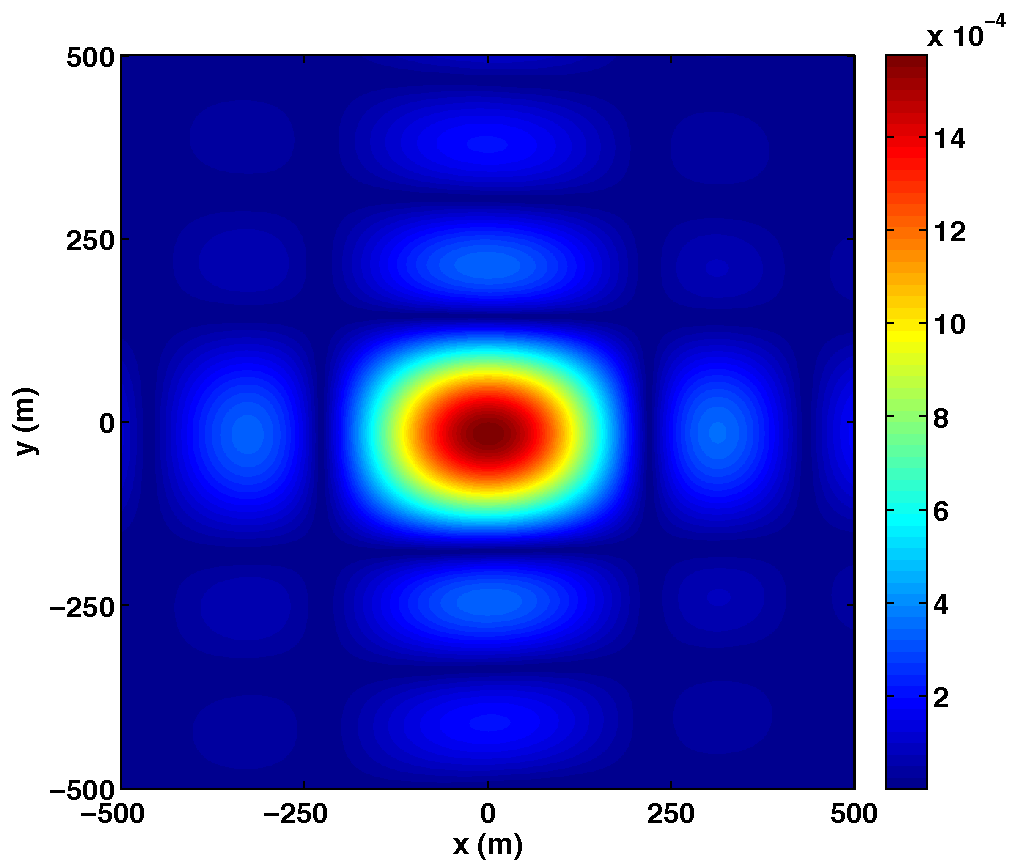
\includegraphics[scale=0.5]{figures/beamfootprint}
  \caption[Circular Bistatic SAR]{This figure shows a monostatic SAR setup where the antenna is traversing a circular flight trajectory. The cone emanating from the aircraft represents the antenna beam pattern.  The oval on the ground represents the beam footprint.}
  \label{fig:flyover}
\end{figure}

